\section{Onde sonore}

\lecture{10}{26 marzo 2024}

Le onde sonore viaggiano in generale in tre dimensioni, oggi ci limiteremo al caso unidimensionale facendole viaggiare in un tubo. Le onde sulla corda sono trasversali rispetto alla direzione di propagazione dell'onda, esse hanno bisogno di qualcosa di solido per propagarsi perché sono necessari dei vincoli sulle posizioni dei punti. Nei liquidi e nei gas le onde trasversali non sono quindi possibili, mentre avvengono onde longitudinali (oscillazione nella stessa direzione del moto).
Se ho una direzione di propagazione ben precisa le onde sono trattabili a tutti gli effetti come onde scalari.
\begin{figure}[H]
	\centering
	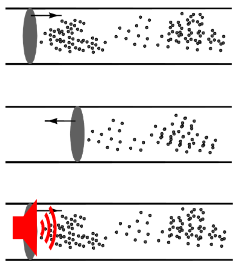
\includegraphics[width=0.2\textwidth]{screenshots/2024-03-26-11-17-49.png}
	\caption{Tubo riempito di gas e membrana che possa comprimere o decomprimere il gas. La membrana può essere immaginata come un semplice speaker.}
\end{figure}
L'attivazione del pistoncino provoca variazioni di pressione e quindi di densità del gas. Pongo un sistema di riferimento con \(x=0\) sulla membrana e studio il comportamento del tubo.
\begin{figure}[H]
	\centering
	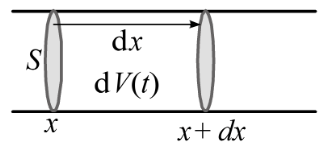
\includegraphics[width=0.4\textwidth]{screenshots/2024-03-26-11-21-58.png}
\end{figure}
Mi limito a una zona del tubo \([x, x+ \mathrm{d} x]\) limitata da due diaframmi senza massa e mobili. La massa \(\mathrm{d} m\) del gas occupa nel tempo volumi diversi, ma è una costante. Inizialmente \(\mathrm{d} m = \rho _0 D \mathrm{d} x\). Successivamente il gas viene compresso e i due diaframmi si muovono.
\begin{figure}[H]
	\centering
	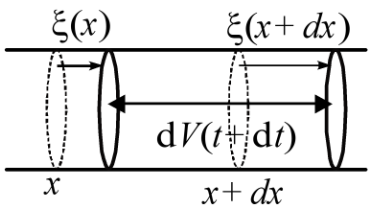
\includegraphics[width=0.4\textwidth]{screenshots/2024-03-26-11-25-08.png}
\end{figure}
Quindi ho che
\begin{gather}
	\mathrm{d} V(t) = S [\mathrm{d} x + \xi (x + \mathrm{d} x) - \xi (x)]=S \mathrm{d} x \left[ 1 + \left( \frac{\partial \xi }{\partial x}  \right)_x  \right]\\
	\mathrm{d} m = cost. \implies \rho _0 S \mathrm{d} x = \rho S \mathrm{d} x \left[ 1+ \left( \frac{\partial \xi }{\partial x}  \right)_x \right]\\
	\rightsquigarrow \frac{\rho}{\rho _0} = \frac{1}{1+ \left( \frac{\partial \xi }{\partial x}  \right)_x}
\end{gather}
Ora posso espandere per piccole perturbazioni:
\begin{gather}
	\frac{\rho }{\rho _0} = \left[1+ \left( \frac{\partial \xi }{\partial x}  \right)_x  \right] ^{-1} \thickapprox 1 - \left( \frac{\partial \xi }{\partial x}  \right)_x\\
	\rightsquigarrow \rho (x,t) - \rho _0 = - \rho _0 \left( \frac{\partial \xi }{\partial x}  \right)_x 
\end{gather}
Studiamo la dinamica del volumetto sull'asse x. \(a_x = \frac{\partial ^{2} \xi }{\partial t ^{2} } \). Sia \(p(x)\) la pressione.
\begin{equation}
	F_x = p(x)S - p(x+ \mathrm{d} x)S
\end{equation}
Proseguendo con i calcoli si ottiene che
\begin{figure}[H]
	\centering
	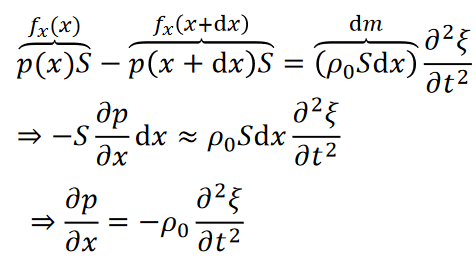
\includegraphics[width=0.4\textwidth]{screenshots/2024-03-26-11-36-18.png}
\end{figure}
Ho collegato una variazione del gas (pressione) a una variazione del mio volumetto. Quindi le onde sonore cambiano la pressione \(p(x)\) e la densità \(\rho (x)\). Adesso studio la variazione di \(p(\rho )\) in prossimità della condizione di equilibrio \((P_0=p(\rho _0), \rho _0)\):
\begin{equation}
	p(\rho )\thickapprox P_0 + \left. \frac{\partial p}{\partial \rho } \right| _{\rho = \rho _0}(\rho - \rho _0) = P_0 + \frac{\beta }{\rho _0}(\rho - \rho _0) = P_0 - \beta \left( \frac{\partial \xi }{\partial x}  \right) _x
\end{equation}
Devo capire quanto vale \(\beta / \rho _0\). Possiamo assumere che il gas faccia una trasformazione adiabatica, perché le trasformazioni che comportano un passaggio di calore sono molto lente e le onde sonore sono invece molto veloci. Grazie a questa considerazione possiamo scrivere \(p(\rho ) = \alpha \rho ^\gamma \).
\begin{gather}
	\beta = \rho _0 \left. \frac{\partial p}{\partial \rho } \right| _ {\rho = \rho _0} = \rho _0 \gamma \alpha \rho _0 ^{\gamma -1} = \gamma \alpha \rho _0 ^\gamma = \gamma P_0\\
	p(x) = P_0 - \beta \left( \frac{\partial \xi }{\partial x}  \right) _x \rightsquigarrow \frac{\partial p}{\partial x} = - \beta \left( \frac{\partial ^{2} \xi }{\partial x^{2} }  \right) _x
\end{gather}
Da cui si ottiene un'equazione di D'Alembert:
\begin{figure}[H]
	\centering
	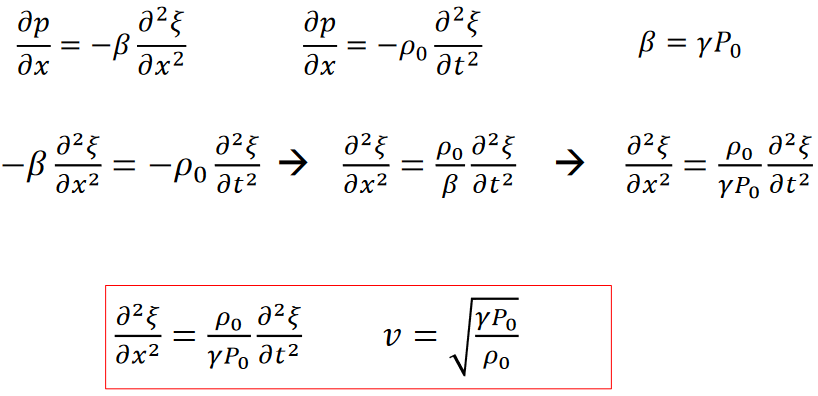
\includegraphics[width=0.6\textwidth]{screenshots/2024-03-26-11-51-20.png}
\end{figure}
Le soluzioni sono le stesse di quelle viste sulla corda! In particolare, avremo onde regressive e progressive.
\begin{eg}
	Verifichiamo la previsione teorica della velocità del suono considerando l'aria secca a livello del mare: \(P_0 = 1.015 \times 10^5 \unit{Pa},\ \rho _0 = 1.29 \unit{kg/ m^3 }\). \(\gamma \) è praticamente 1.4 perché l'aria è principalmente un gas biatomico (azoto e ossigeno).
	\begin{equation}
		v_{teo} = \sqrt{\frac{\gamma P_0}{\rho _0}} = 331 \unit{m/s} \hspace{1cm} v_{mis} = 330 \unit{m / s} 
	\end{equation}
	C'è un accordo entro il 3 per mille! Significa che le approssimazioni che abbiamo fatto sono valide e funzionano molto bene. In acqua la velocità è di circa \(1400 \unit{m / s}\), nel granito è circa \(6000 \unit{m /s}\).
\end{eg}

\paragraph{Cosa sono le onde sonore?}
Sono onde di spostamento della posizione delle molecole \(\xi (x,t)\):
\begin{equation}
	\frac{\partial^{2}  \xi }{\partial x^{2} } = \frac{\rho _0}{\gamma P_0} \frac{\partial ^{2} \xi }{\partial t ^{2} }  
\end{equation}
Ma sono anche onde di densità \(\rho (x,t)\):
\begin{equation}
	\rho (x,t) = \rho _0 - \rho _0 \frac{\partial \xi }{\partial x} \rightsquigarrow \frac{\partial ^{2} \rho }{\partial x^{2} } = \frac{\rho _0}{\gamma P_0} \frac{\partial ^{2} \rho }{\partial t ^{2} }  
\end{equation}
E anche onde di pressione \(p(x,t)\):
\begin{equation}
	p(x,t) = P_0 - \gamma P_0 \frac{\partial \xi }{\partial x} \rightsquigarrow \frac{\partial ^{2} p}{\partial x^{2} } = \frac{\rho _0}{\gamma P_0} \frac{\partial ^{2} p}{\partial t ^{2} }  
\end{equation}
